% outline introduction
% 1. Reinforcement learning introduction
% 2. games as virtual learning environment
% 3. Research approach
% 4. Structure of the Dissertation

\chapter{Introduction}

Artificial Intelligence is an extremely interesting but difficult problem to
address, as research has to at least account for the complexity and breath of
behaviour that has been shown in animals and humans. Autonomy can be sometimes
programmatically engineered, but most of intelligent behaviour requires some
amount of learning that can only be acquired through direct interaction with the
environment, as a big part of being ``intelligent'' has to do with the ability
to generalise knowledge and behave reasonably in unseen scenarios.

\section{Reinforcement Learning}

A technique developed specifically to address this type of learning process is
Reinforcement learning. Reinforcement learning provides a general framework to
learn behaviour in a goal-oriented fashion and without requiring expert
knowledge or labelled data. It is framed to be functional even in situations
where reward is delayed and where environments are not deterministic. Because of
its foundations on dynamic programming, it also allows the use of rich and
powerful mathematical tools for its analysis. Unfortunately those algorithms
learn more or less good behaviour sets only when the environment is sufficiently
tractable, and they start breaking down as the state space increases in size. To
study reinforcement learning we therefore need testbeds that allow to
parametrise the size of this state and that remain interesting enough to provide
challenges for current state-of-the-art algorithms.

\section{Games as Virtual Learning Environments}

The idea of using games as testbeds for Artificial Intelligence is not a new
one. Board games such as Chess, Backgammon and Go have been historically linked
to challenges in AI research, and the AI community has used those games to
compare and study the properties of different algorithms. During the past couple
of decades, the community has gradually ``solved'' or fully tackled those board
games, so part of the community shifted to more complex games, most of which
were popular video games. Those already provided the community a perfect excuse
to study search algorithms and symbolic solvers because of the need to challenge
human players, so it's only natural the gradually got integrated as part of the
testbeds used by researchers working in machine learning and more generally
artificial intelligence.

Reinforcement Learning algorithms have since the beginning found usage when
applied to fields such as robot control, natural language processing and
economics, but most of the theoretical work has required relatively simple and
scalable testbeds to compare algorithms in a systematic and rigorous manner.
Most of those domains were simple adaptations of classical AI problems such as
grid worlds and bandit problems, but as research started getting past those
problems the community had to come up with more structured and complex domains.
Those testbeds have historically mostly consisted of board games like go and
backgammon, but in the past couple of decades the community has also introduced
domains such as simulated football and a variety of video games. All of those share
characteristics that make naive reinforcement learning complex to engineer and
train: they can possess large action or environment state sets, they challenge
algorithms by providing only a degree of partial of observability or they can be
properly solved only by obtaining very strong long-term strategies (that realms
such as planning try to tackle).

\begin{figure}[h]
    \centering
    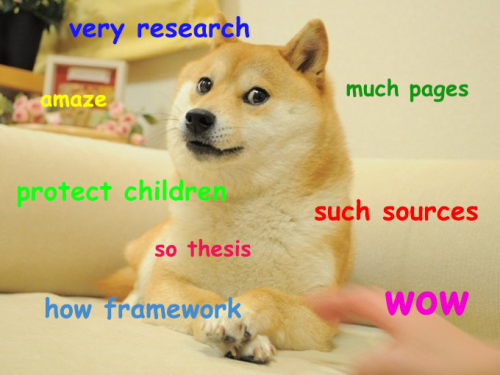
\includegraphics[width=\textwidth]{placeholder}
    \caption{The ATARI Learning Environment.}
    \label{fig:ALE}
\end{figure}

A popular and recent learning platform has been for instance the Atari Learning
Environment (ALE), which researchers have mostly used to study reinforcement
learning algorithms that can learn a variety of policies for different games.
Unfortunately the majority of the games contained in this particular
platform don't require anything way more complex than reactive policies, which
means that studying more advanced policy learning on those games has become
quite a forced process.

A category of video games more suitable for providing complex scenarios for
studying RL is the category of Real-Time Strategy (RTS) games. This typology of
games generally requires some amount of long-term planning combined with
interactive and generalisable short-term or reactive planning, and it's
particularly challenging to reinforcement learning algorithms because of the
intrinsic partial observability, the unusually big action space, and its nature
of competitive game. We focus on one of the most popular and still widely played
RTS games, Starcraft.

% cite from http://umichrl.pbworks.com/w/page/7597597/Successes%20of%20Reinforcement%20Learning

\section{Approaching the problem} % TODO rename

The point of this work was primarily about exploring what it would take to
concretely transform and use StarCraft as a platform to study reinforcement
learning and general artificial intelligence. We adopted a scoping approach to
deal with the engineering problem, with the goal to reach a state where we could
successfully run state of the art learning algorithms on StarCraft. This
therefore required the construction of a robust and generic interface to the
game, the creation of an interface to one of the popular tensor libraries and
finally porting and testing a few basic reinforcement learning and deep
reinforcement learning algorithms.

The idea was to prove the feasibility of using StarCraft as a learning platform,
to release the first version of a useful interface to allow the community to
bootstrap work on real time strategy games, and to create a baseline for later
work in the area.

\section{Report Structure}

Chapter 2 presents reinforcement learning and discusses some of the research
done by games. It outlines properties of real time strategy games and it seeks
to explain the benefits of using StarCraft as a research platform. Chapter 3
presents the engineering approach taken and the developed architecture, covering
the entire pipeline from the game to the agent interface, also providing some
example agent learning algorithms. Chapter 4 presents results obtained from
testing the platform using a couple of model-free reinforcement learning
algorithms. Finally Chapter 5 discusses some improvements for the design and
future work.
